% Lines that start with a % are comments and are not included when the LaTeX file is converted to a pdf

% Set up the document class - this can be changed if a different format is required 
\documentclass[12pt,a4paper,twoside]{article}

% Include packages that contain additional features, for example including special mathematical characters and images in your document
\usepackage{amssymb,amsmath,graphicx}

% The beginning of the document...
\begin{document}

% Please change the following accordingly...
\centerline{\large Exercises sheet 1}\vspace{0.5em}
\centerline{\large by Maximilian Richter and Christian Heppe}\vspace{2em}

% Split the different exercises into different sections...
\section*{Exercise 5}

% To include a plot it must be in the same directory as the .tex file.
a) (Orange) and b) (Blue)\\
% Remove the "%" in the following line and change the "plot.png" to the name of the plot to include.
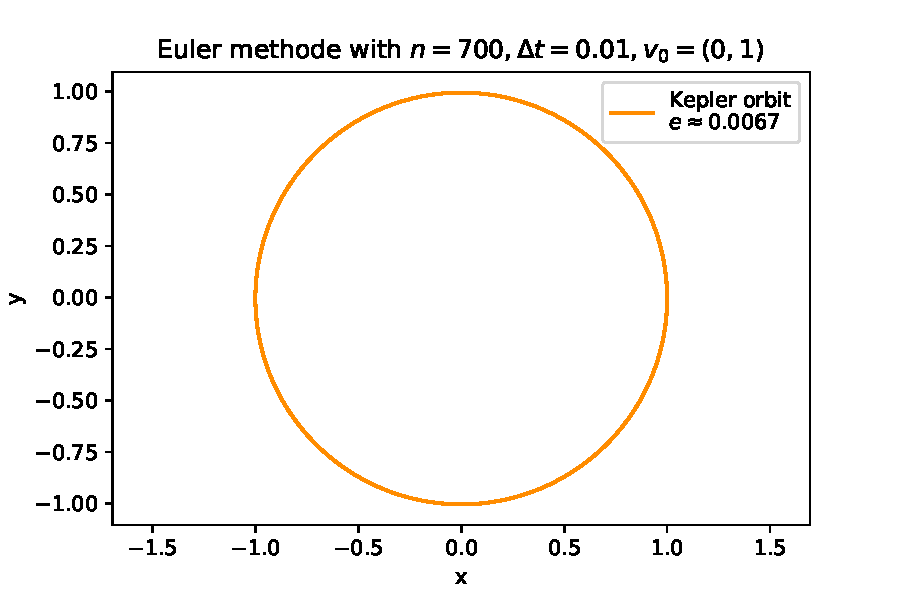
\includegraphics[width=8cm]{euler.pdf}
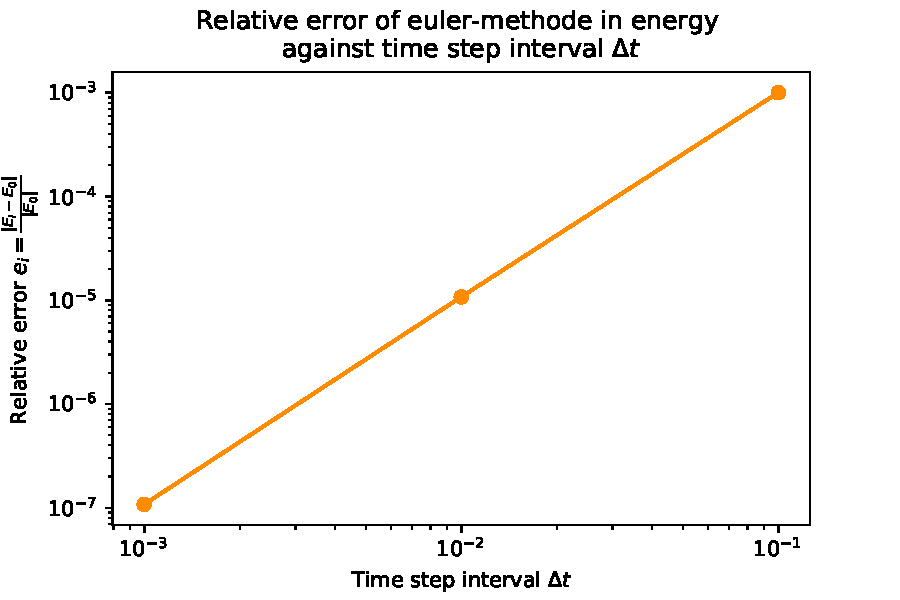
\includegraphics[width=8cm]{error_euler.pdf}
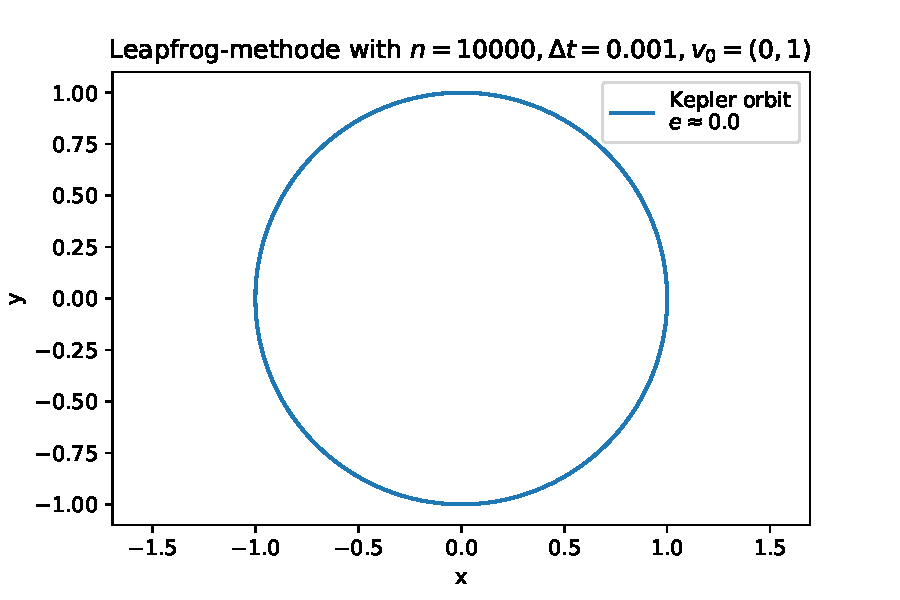
\includegraphics[width=8cm]{leap.pdf}
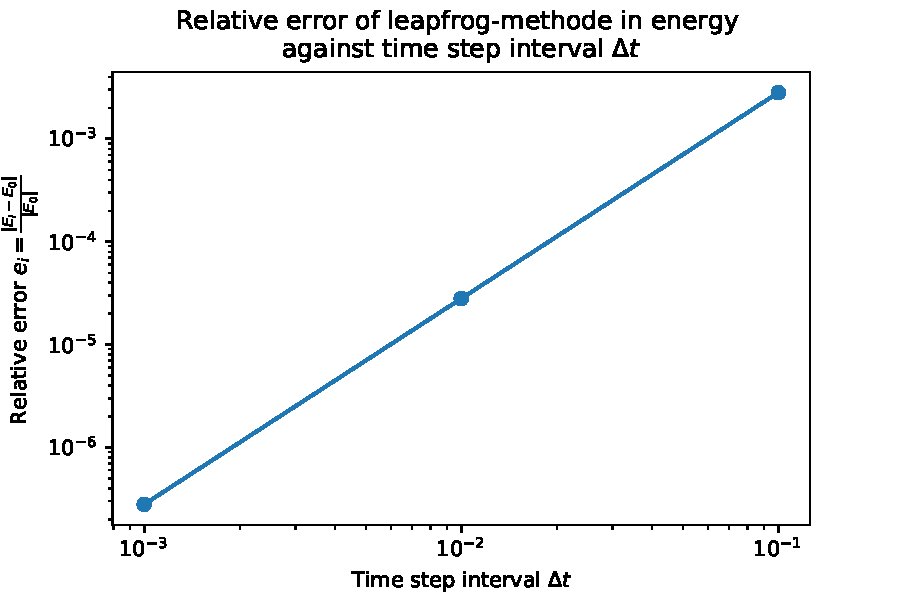
\includegraphics[width=8cm]{error_leap.pdf}
\newline
\newline
In order to test the euler and the leapfrog methode, we evaluated the energy and compared the final energy with the initial energy for 3 different eccentricites (in our case we did that in a for-loop with different steps and timeintervalls (stepsizes)). \\
Both methodes satisfy our expectations pretty good, as expected, the relative error of the energy vanishes exponentially as we decrease the stepsize $\Delta t$ logarithmically. 
For further details see the python-code in the appendix.
\end{document}

